\newgeometry{total={210mm,297mm},left=20mm,right=20mm,bindingoffset=5mm, top=25mm,bottom=25mm} 
\begin{partwithabstract}{Problem Introduction \& Motivation}
    The objective of this project is the development of a model for the automated vertebrae instance segmentation of \acrshort{mri} and \acrshort{ct} scans of the lumbar part of the human spine based on point annotated training data.
    
    This part of the book aims to clarify these terms. 
    I start off with some information regarding the human spine and the medical imaging techniques to investigate it.
    Secondly, I define and clarify different machine learning problems and techniques when working with two and three dimensional images.
    This part of the book ends with a discussion of previous work. 
    First the previous work to tackle the problem of instance segmentation of the human spine from medical images.
    Then prevous work in the field of \Gls{weaklysupervisedl} \Gls{machinevision}.
\end{partwithabstract}

\restoregeometry
\chapter{The human spine}\thispagestyle{empty}
\par{
    This document presents a model for automatic segmentation of \acrfull{ct} and \acrfull{mri} images of the lumbar spine.
    This chapter introduces these terms\footnote{This work is not a medical desideration. For in-depth knowledge on the anatomy and physiology of the spine, consult the specialized literature.}.
    Secondly, it gives a basic overview of the medical imaging techniques. 
    Finally, it touches upon a specific medical procedure in which this information is used: the minimally invasive surgery of a spinal hernia.
}
\section{Anatomy of the human spine}

\par{
    The spinal column, vertebral column or backbone\footnote{NL: \textit{wervelkolom}} is a structure of 34 bones. 
    It holds the body upright while providing it with the mobility to bend and twist.
    the \textit{intervertebral discs} make this possible. These consist of a ring of fibrocartilage and an inner gel-like centre and form an articulation between two vertebrae.
    Moreover, the vertebral column serves as a conduit for significant nerves running from the brain to the toes.
    The spinal column, as illustrated in figure \ref{fig:spineimage} can be divided into five regions:
}
\begin{description}
    \item[the Cervical spine:] 7 vertebrae of the neck, indicated by $C1$ to $C7$\footnote{Vertebrae are numbered from the head down. C1 (\textit{atlas}) is the vertebra closest to the head}.
    \item[the Thoracic spine:] 12 vertebrae of the middle back ($T1$ to $T12$).
    \item[the Lumbar spine:] 5 vertebrae that form the lower back. These are commonly referenced as $L1$ to $L5$.
    \item[the Sacrum:]\footnote{NL: \textit{Heiligbeen}} This is a structure consisting of 5 naturally fused vertebrae ($S1$-$S5$).
    \item[the Coccyx:]\footnote{NL: \textit{Stuit of staartbeen}} Structure of 3 to 5 naturally fused vertebrae at the end of the spinal column.
\end{description}


\begin{SCfigure}[][h!]
    \centering
    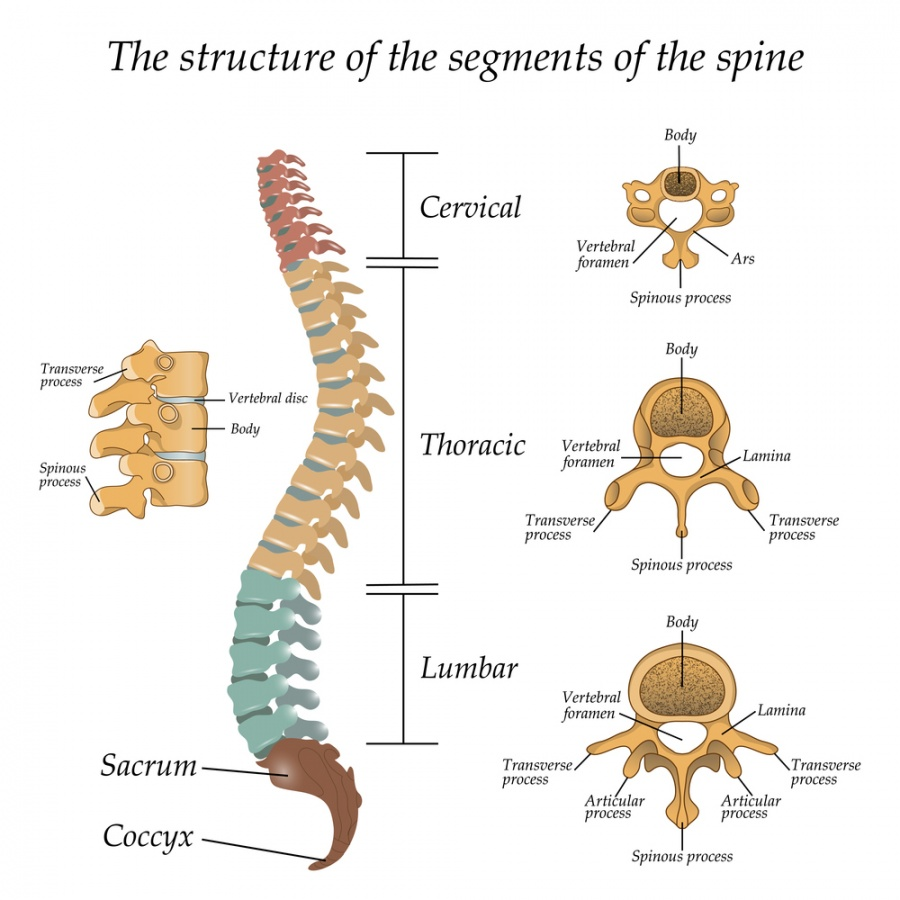
\includegraphics[width=10cm]{/home/thesis/images/SpineModel.jpeg}
    \caption{\label{fig:spineimage}Model of the human spine. The five vertebrae in green form the lumbar spine. They are referred to as \textit{L1} to \textit{L5} from top to bottom. Image source: \url{shutterstock.com}}
\end{SCfigure}

\section{Pathologies of the human spine}
\par{
    This document does not aim to provide an exhaustive list of all human spinal pathologies. 
    Two pathologies are interesting to discuss further as an introduction to this work since they occur in the data used in this project (see page \pageref{sec:datasets} for further details).
}
\begin{SCfigure}[][h!]
    \centering
    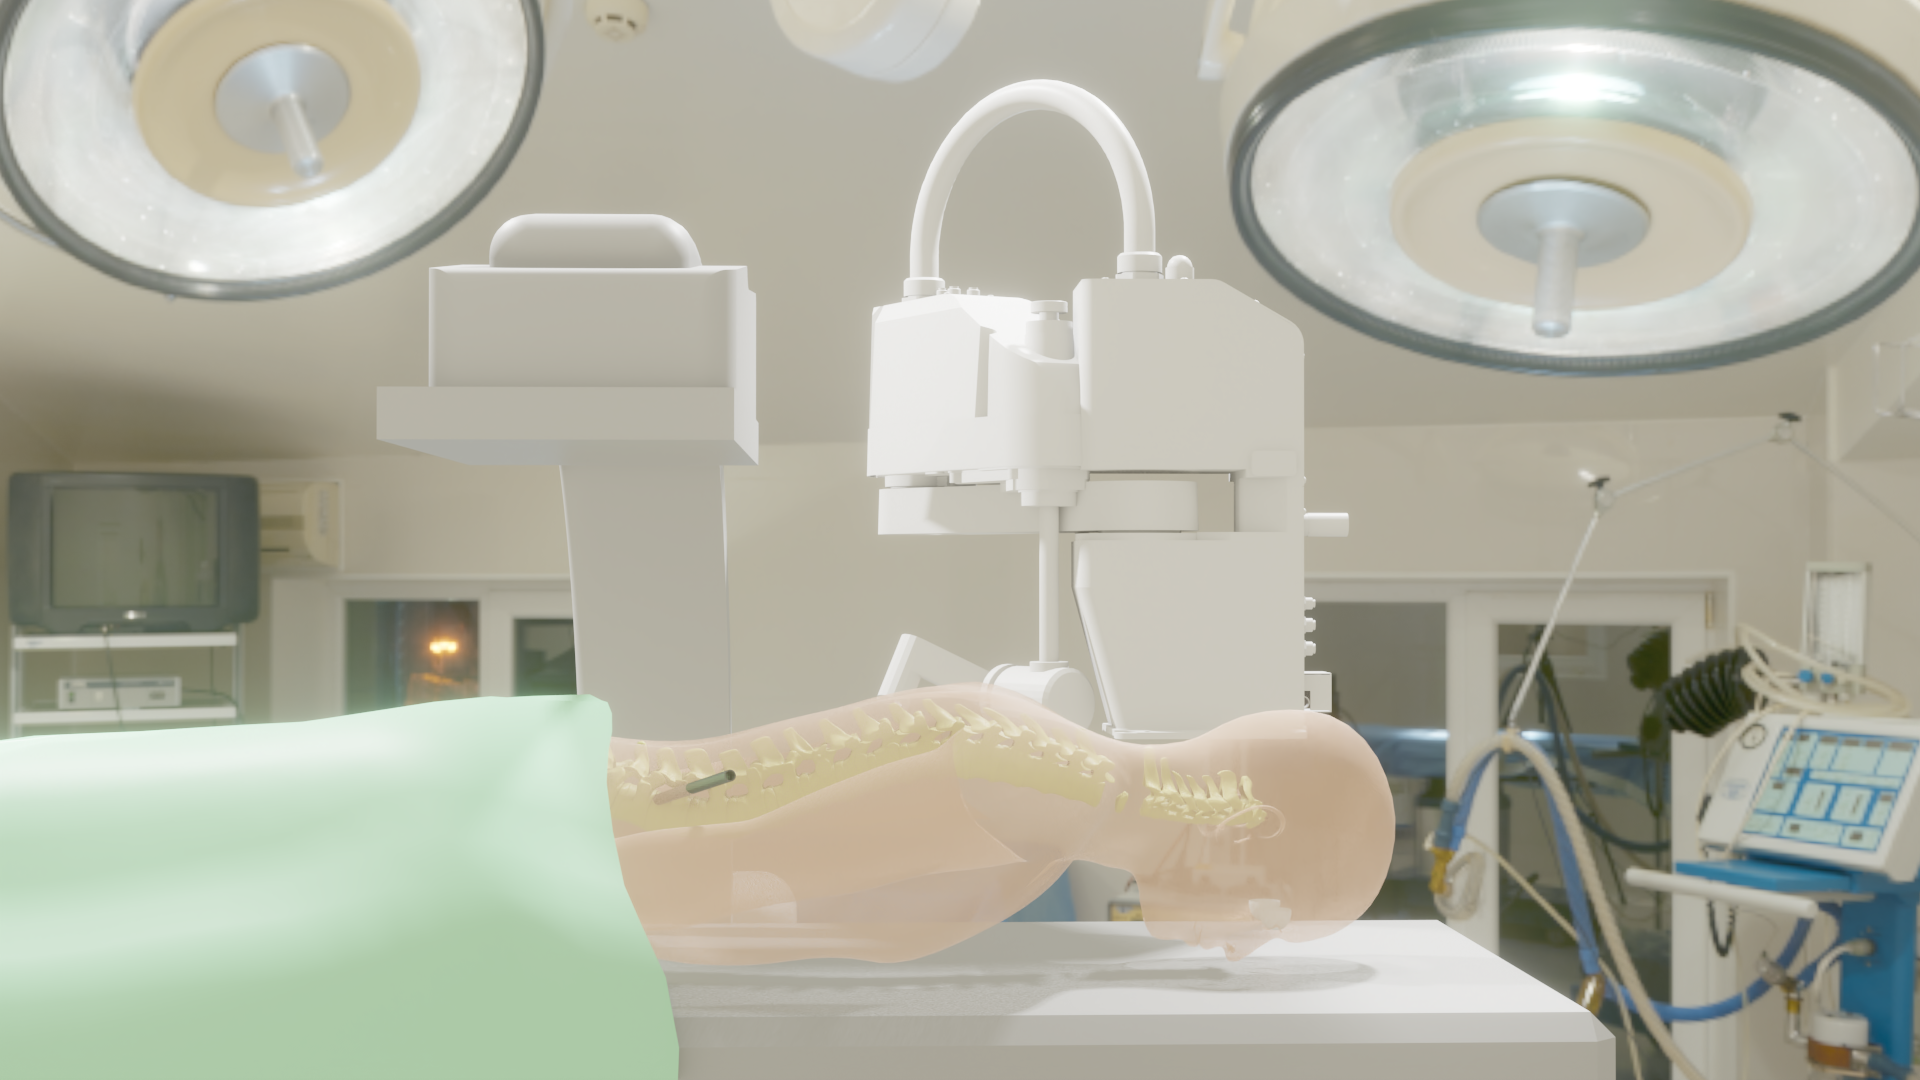
\includegraphics[width=10cm]{/home/thesis/images/REISS_illustration.png}
    \caption{Artist's impression of the start of the surgical treatment of a lumbar hernia. 
    This image shows the dilator through which the surgical instruments will be inserted to mill away the bulging disc material.
    This procedure requires repeated visualization of the instruments and the spine via X-ray images. \textit{This illustration is designed by Verhaert NP\&S}.\label{fig:REISS_procedure}}
\end{SCfigure}
\par{
    First, there is \textit{scoliosis}, which is a sideways curve of the spine.
    The severity of this condition can vary from relatively mild to severe. 
    In severe cases, scoliosis can affect the patient's movement and breathing.
}
\par{
    Second, there is the \textit{spinal hernia} or spinal disc herniation\footnote{Spinal disc herniation is sometimes referred to as a \textit{slipped disc}.}. 
    A spinal hernia is caused by damage to the \textit{annulus fibrosus}\footnote{The fibrocartilage ring around the softer gel-like centre of the intervertebral disc.}. 
    This damage can cause the intervertebral disc to bulge out. 
    This condition is painful due to the inflammation reaction, and in severe cases, the bulging material can irritate or cause impingement of the critical nerves along the spine.
    The nerve impingement can even lead to radiating pain to the limbs or even limb paralysis.
    In severe cases, a spinal hernia requires surgical treatment.
    This specialized procedure requires repeated medical imaging to allow the surgeon to accurately investigate the situation before the operation and assure correct positioning of the instruments during the intervention.
}
\par{
    In image \ref{fig:REISS_procedure}, the start of the surgical treatment procedure for a lumbar hernia is illustrated.
    One possible benefit of improved automatic interpretation of \acrshort{mri} and \acrshort{ct} scans is providing support for this procedure.
    This delicate procedure requires interpreting and registering information from both scan types (at different times), a demanding task for which automated support could be helpful.
    Image registration of the pre-operative \acrshort{mri} scan with the operation planning to the imaging of the situation on the operation table starts by segmentation of the affected vertebrae.
}

\section{Medical imaging of the human spine\label{sec:medical_imaging}}
\marginpar{
        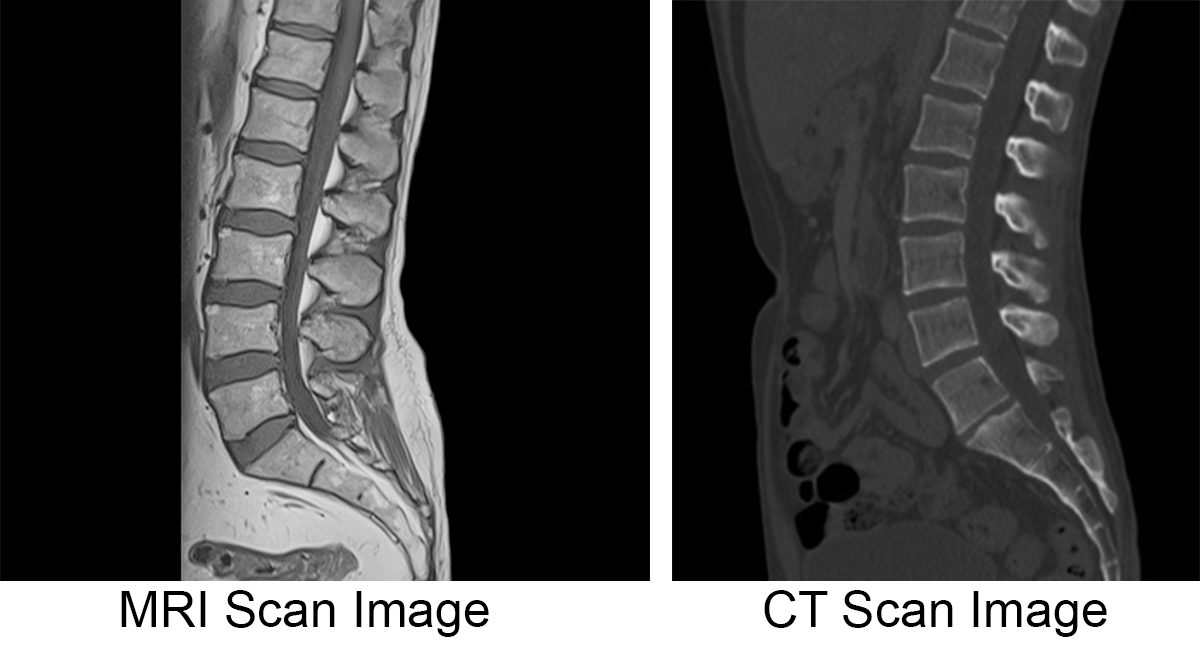
\includegraphics[width=5cm]{/home/thesis/images/MRI_CT_images.jpeg}
        \captionof{figure}{Illustration of \acrshort{ct} and \acrshort{mri} images of a human lumbar spine.}
        \label{fig:mri_ct}
    }
\par{
    For diagnosis and visualization of spinal pathology several medical imaging techniques are used: \acrfull{ct}, \acrfull{us} and \acrfull{mri}. 
    These techniques allow non-invasive visualization of the spine and discs in three dimensions.
    Slices from volumetric scans (\acrshort{mri} and \acrshort{ct}) are illustrated in \ref{fig:mri_ct}.
}

\subsection{CT scan}
\par{
    The \acrfull{ct}\footnote{Also known as CAT-scan, for Computed Axial Tomography or Computer-assisted Tomography.} is a non-invasive medical imaging procedure
    \footnote{\Gls{tomography} scans are primarily used for medical purposes. 
    It is also used in the industry for non-destructive inspection of components and assemblies.
    In geology, it is used to identify materials in a drill core quickly. In archaeology, it is used for the non-destructive investigation of artefacts. } 
    for diagnostic purposes. 
    A \acrlong{ct} procedure consists of the combination of an array of X-ray attenuation images taken with a rotating X-ray tube as illustrated in figure \ref{fig:CT_principle}. 
    These images can be combined with a \Gls{tomography} algorithm to reconstruct a volumetric representation of the radiographic density.
}
\par{
    Contrary to \acrfull{mri} imaging, this technique is suitable for patients with a pacemaker or insulin pump since there are no magnetic fields involved.
    The main disadvantage of \acrshort{ct} is the exposure to ionizing radiation\footnote{Radiation exposure increases the probability of cancer.} of the patient and the risk of exposure of the medical professional to the same radiation.
    The image quality increases with radiation dose, but so does the radiation exposure.
    Improving the reconstruction algorithms to obtain higher-resolution images while reducing radiation is an ongoing area of research. 
}
\marginpar{
        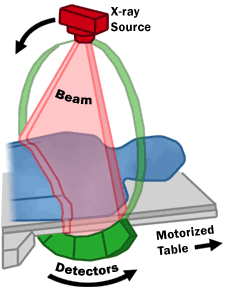
\includegraphics[width=5cm]{images/FDA_CT_Scan.png}
        \captionof{figure}{Conceptual illustration of the working of a \acrlong{ct} scan. Image from \url{www.fda.gov/radiation-emitting-products/medical-x-ray-imaging/computed-tomography-ct}}
        \label{fig:CT_principle}
    }

\subsection{MRI scan}
\par{
    The \acrfull{mri} scan is a medical imaging technique that is not based on ionizing radiation\footnote{Eventhough the alternative name \textit{nuclear} magnetic resonance (NMR) might confuse.}.
    \acrshort{mri} imaging will visualize the concentration of hydrogen\footnote{In theory, other atoms than hydrogen can be excited by adapting the excitation frequency.} atoms.
    The patient is positioned in a tunnel where a high constant magnetic field is applied. 
    A temporary oscillating signal is applied with the resonance frequency corresponding to hydrogen atoms is superposed on the static magnetic field.
    The hydrogen atoms will fall back to the equilibrium state, emitting radiofrequency (RF) signals, measured by receiving coils.
    \acrlong{mri} is particularly suitable for visualization of tissue with higher water content, such as tumours and infections, and to visualize fat.
}
\par{
    An \acrshort{mri} scan can be \textit{T1 weighted} or \textit{T2 weighted}. 
    A T1 weighted image is constructed based on the relaxation time of the magnetization is colinear with the direction of the static field
    while T2 weighted images are based on the magnetization perpendicular to the static field.
    While areas with higher water content, such as infected areas, will release a higher signal on a T2-weighted \acrshort{mri} scan, the same images will show a lower signal strength for T1-weighted scans.
}
\par{
    Contrary to \acrfull{ct} scans, the \acrlong{mri} procedure does not expose the patient of radiation. 
    Due to the high magnetic fields, the technology cannot be used for patients with pacemakers, cochlear implants or other metallic objects in the body.
    \acrshort{mri} allows to visualize soft tissue better than \acrshort{ct} images. An \acrshort{mri} image allows visualizing both the grey and white brain matter, while this is not possible with \acrshort{ct} images.
    Although both techniques produce images that resemble each other, none can replace the other one completely.
}


\chapter{Machine vision}

\Gls{machinevision} is the branch of \Gls{ai} focussed on image processing.
The machine vision task performed in this work is called instance \Gls{segmentation}.
In this chapter, I explain what this means. 
The task of segmentation is compared to other machine vision tasks.

This work investigates the used of \Gls{weaklysupervisedl} data for training an Instance segmentation model. 
The concept and benefits of \Gls{weaklysupervisedl} machine learning are explained.

\section{Machine vision tasks \label{sec:machinevisiontasks}}

\Gls{machinevision} is a broad discipline. 
Humans extract information from images almost subconsciously and we are often not aware of the different tasks we perform on images.
The objective of this section is to briefly define different machine vision tasks discussed further in this book. 
Several machine vision tasks consist of \textit{recognizing} objects, animals or humans in an image.
A model is build for a finite list of \textit{categories} that can be present in an image.
Depending on the question asked ad inference time, on can distinquish the following tasks.

\begin{description}
    \item[Image classification] is the task of determining what object category\footnote{or categories} is present in the image. Is there a cat in this image?
    \item[Object counting] is the task of counting how many instances of each category can be seen in the image. How many cats are there in this picture? 
    \item[Object detection] consists not only of identification of the object. Also the spatial position is requested. This is often requested in the form of a bounding box. Where is the cat in this picture, if a cat is present?
    \item[Semantic segmentation] requires that for each image pixel, a class is estimated. Pixels that do not belong to a specific class are called the \textit{background}.
    \item[Instance segmentation] requires not only that the semantic class is determined for each pixel, but also that two individuals of the same class\footnote{say, two cats.} are distinguished.   
\end{description}

The difference between these machine vision tasks is illustrated in figure \ref{fig:machinevisiontasks}. 

\begin{SCfigure}[][h!]
    \centering
    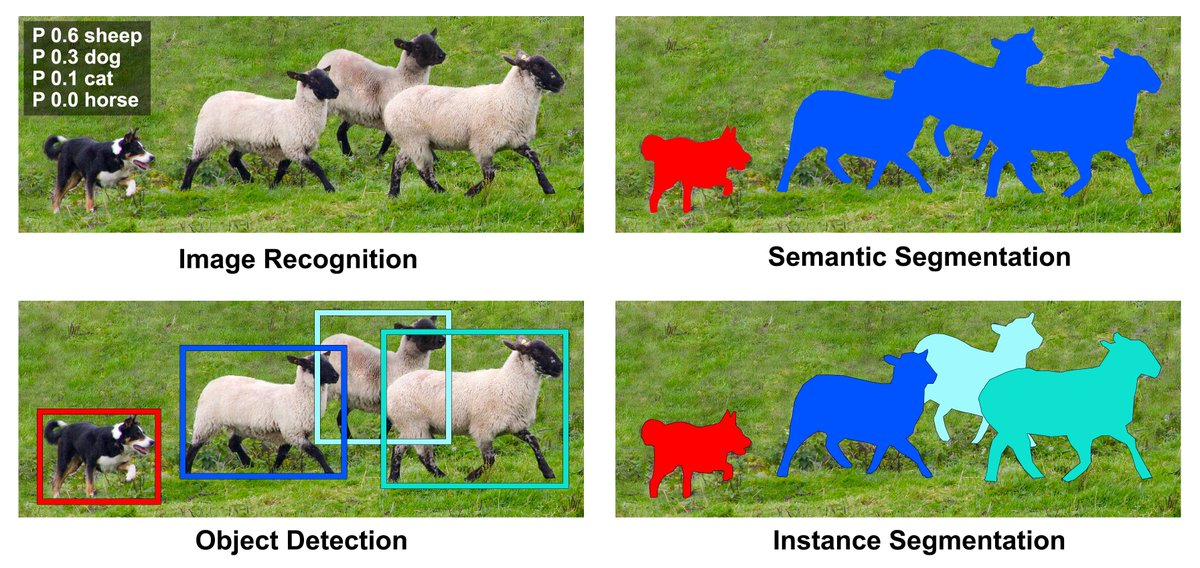
\includegraphics[width=10cm]{/home/thesis/images/Classification_vs_Segmentation.jpg}
    \caption{Illustration to compare different Machine vision tasks \cite{SemTorch76:online}. 
    Object detection means that the location of several objects is estimated by the model. This is indicated by the \textit{bounding boxes}.
    Segmentation of an image is the process of classifying each pixel in the correct class or assign it to the \textit{background} class.
    Semantic segmentation makes no difference between different instances of the same semantic class, instance segmentation does.
    \label{fig:machinevisiontasks}}
\end{SCfigure}

Other interesting applications of \gls{machinevision} include\footnote{This list is not exhaustive.}:
\begin{description}
    \item[Face recognition] is the identification of human faces. 
    \item[Image reconstruction] or \textit{inpainting} consists of recreating parts of a damaged image.
    \item[Image captioning] consists of the creation of full sentences describing the content of an image.    
\end{description}



\section{Supervision types}

To build a model to perform the tasks discussed in \ref{sec:machinevisiontasks}, this model needs to be trained.
This requires a set of \textit{labelled} images. 
This means that a collection of images needs to be provided where an expert in the intended task has provided correct information the model can \textit{learn} from.
Depending on the model objective, other types of labelling are required.
Figure \ref{fig:ImageLabelTypes} illustrates several types of image supervision : 
Point supervision, squiggle, bounding box and full mask.
The generation of these labels is very expensive and time-consuming.
Especially \gls{deepl} models are known to be very data-hungry. 
These models have determined unprecedented performance, provided sufficient data has been provided.

\begin{SCfigure}[][htb]
    \centering
    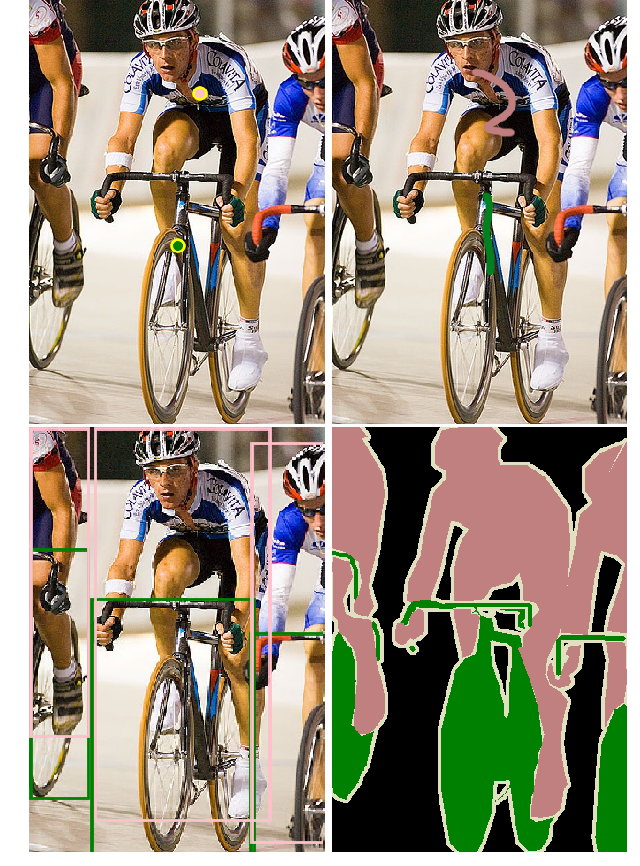
\includegraphics[width=10cm]{/home/thesis/images/McEver.png}
    \caption{Four different annotation types \cite{McEver2020}: 
    On the top left the picture is point level annotated. The points are inflated for visibility.
    On the top right, squiggle annotation is used.
    The bottom left shows bounding box supervion.
    While the bottom right image is fully annotated.
    An image level label would indicate that there are multiple instances of \textit{person} and \textit{bike} in the image.
    \label{fig:ImageLabelTypes}}
\end{SCfigure}

Given the high labelling cost, several researchers have investigated ways to train computer vision models with cheaper labels.
This branch of research is known as \Gls{weaklysupervisedl}.
The objective is to construct a strong model based on \textit{cheap} (incomplete, noisy or imprecise) labels. 
This is sometimes described as \textit{indirect supervision}.
Numerous creative approaches have been conceived. 
It is impossible to give an exhaustive list of approaches. 
In what follows, I will mainly focus on the approaches I chose to investigate myself, but I will also try to give some hints of the remarkable creativity found in the field.
Since the provided annotations in \Gls{weaklysupervisedl} are not full labels, these are sometimes described as \textit{hints} instead\footnote{
    This is based on the insightfull talk at \url{
        https://youtu.be/4EjYxVVCAaE
    }. For example, the destinction between labels and hints.
}.
The basic concept of \Gls{weaklysupervisedl} is that there are two sources of information to draw from: The hints and the prior knowledge about the problem (Priors).
These \textit{Priors} can be any form of prior knowledge about the object to be segmented\footnote{or any other machine vision task.}.
Priors can be the object size, shape or location, the number of instances, the similarity across images or the similarity with exernal images.

Wether an annotation is considered a \textit{weak label} or a \textit{strong label} depends more on the modellers intend than on the annotation itself. 
Basically, when one aims to construct a model to infer output labels with a higher informative value than the original annotations, these \textit{labels} become \textit{hints}.
Making a model to predict bounding boxes from a dataset annotated with bounding boxes means considering these as \textit{strong labels}. 
If one uses the same dataset to construct a model that predicts pixel-wise masks, you use the labels as \textit{weak labels} or \textit{hints}.

For a segmentation task, weak labels can be:
\begin{description}
    \item[Image level labels]: When only  
\end{description}

\todo[inline]{Motivation of weakly supervised learning --> Difference in annotation time and cost from Bearman and Laradji Covid}
\chapter{Previous work}

This project sits at the intersection of two areas of research. 
First there is the application of \Gls{ai} in medical applications, specifically for segmentation problems.
Then, there is the active area of research of \Gls{weaklysupervisedl} machine learning.

\section{Artificial intelligence for medical applications}

\todo[inline]{Start with short overview of other AI problems (~5 lines)}

\Gls{ai} has proven to be a valuable contribution to medical practice to reduce the burden of repetitive tasks on the medical caregiver.

\todo[inline]{elaborate: ppg to blood pressure - slaapapnue}

\section{Segmentation problems for medical applications}

\todo[inline]{General introduction of U-Net and other medical approaches}

For segmentation tasks, the U-net \cite{Ronneberger2015} is widely used. 
This architecture can be represented by a characteristic U-shape, as the name indicates.
It consists of 

\begin{SCfigure}[][htb]
    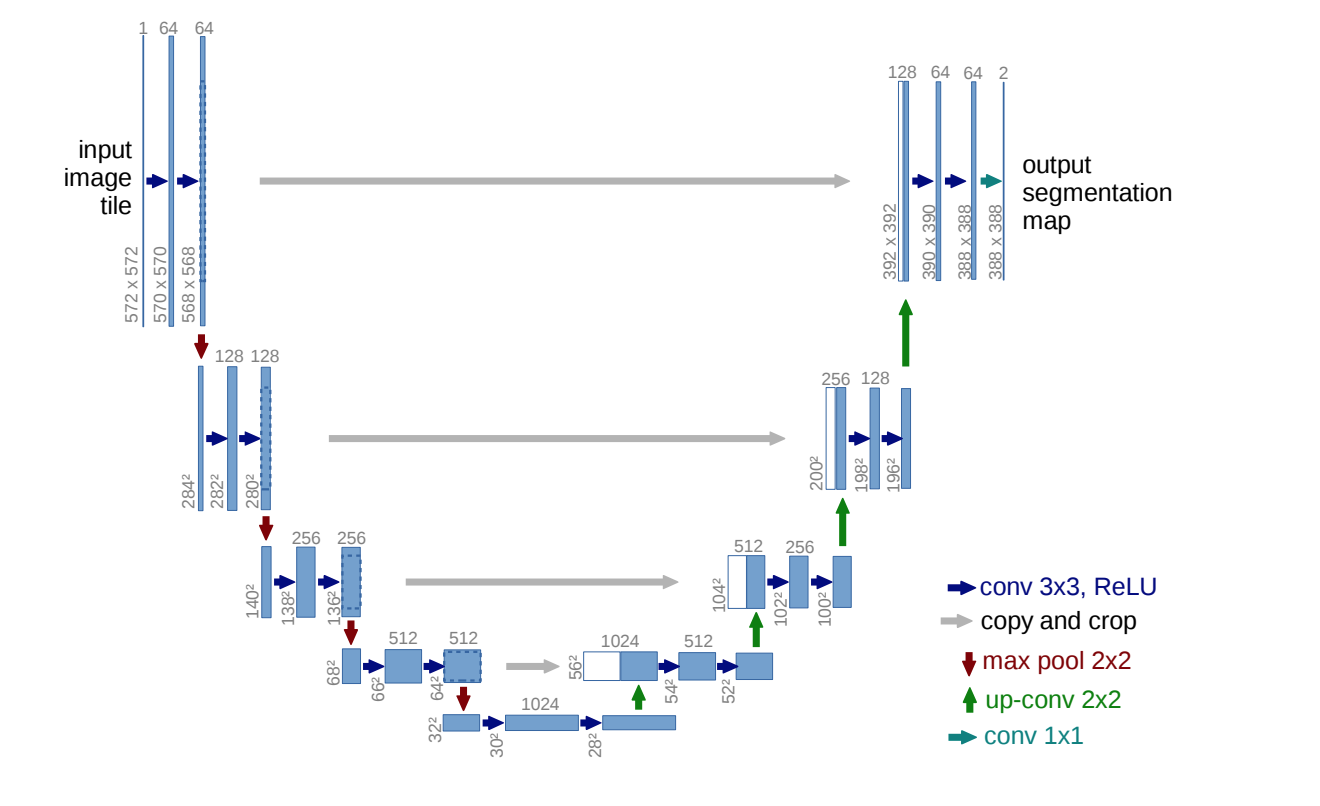
\includegraphics[width=10cm]{/home/thesis/images/UNet_Ronneberger.png}
    \caption{U-Net architecture, as illustrated in \cite{Ronneberger2015}. 
    Each blue box represents a multi-channel feature-map. 
    The number of channels is indicated above the box, the $x \times y$ dimensions are indicated at the bottom left.
    The gray arrows indicate the feature maps in the contracting path are copied and concatenated to the feature maps of the expanding path.}
    \label{fig:unet}
\end{SCfigure}

\todo[inline]{General introduction of U-Net and other medical approaches}

\subsection{Segmentation of the human spine}

\todo[inline]{other authors, approaches --> priors used, metrics used}

\section{Weakly supervised segmentation}

\subsection{General approaches}

\todo[inline]{How is this problem generally solved: PCAMS, WISE, ...}

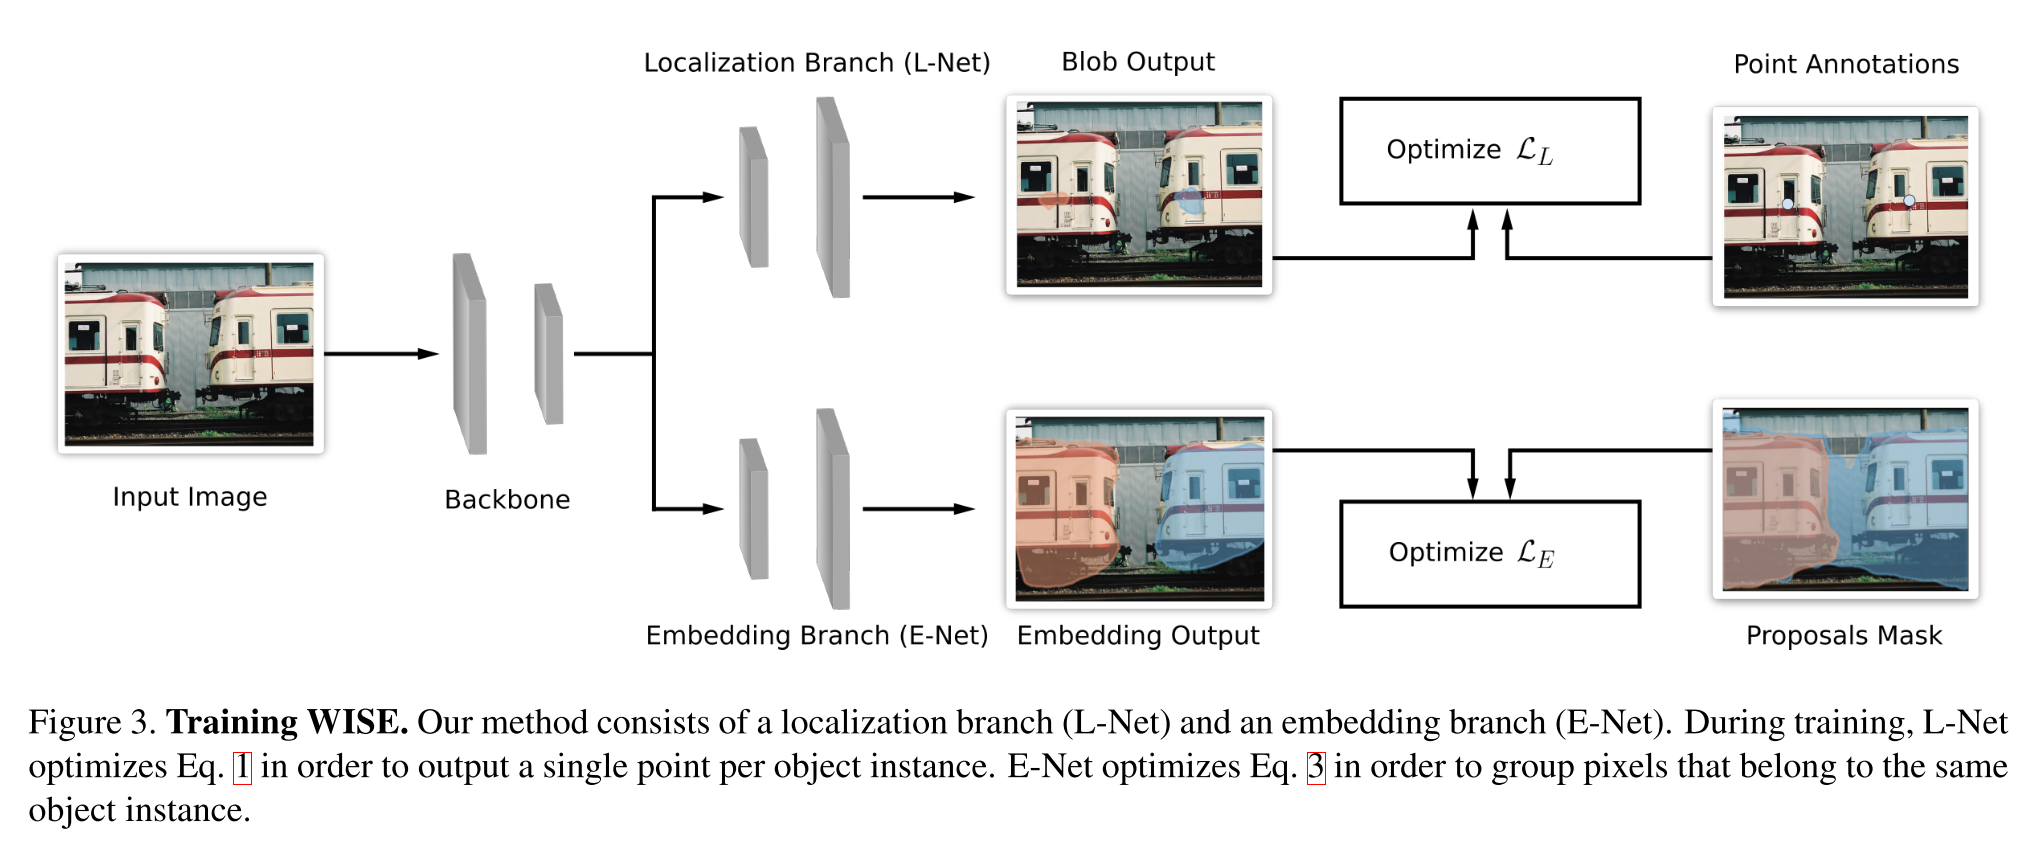
\includegraphics[width=10cm]{/home/thesis/images/Laradji_architecture.png}
\captionof{figure}{Architecture of the U-net based segmentation}
\label{fig:laradji}

\subsection{Weakly supervised segmentation for Medical applications}

Laradji COVID 19
